\documentclass[12pt, a4paper, openany, oneside]{book}
\usepackage[italian]{babel}
\usepackage[T1]{fontenc}
\usepackage[utf8]{inputenc}
\usepackage{amsmath} 
\usepackage{xcolor}
\usepackage{hyperref}
\usepackage[margin=1in]{geometry} 
\usepackage{graphicx}
\graphicspath{{./img/}}
%usepackage[latin1]{inputenc}
\begin{document}
\pagestyle{headings}
\author{\href{https://github.com/daverhapsody}{DaveRhapsody}}
\title{Fisica}
\date{30 Settembre 2019}
\maketitle
\tableofcontents
\chapter{Introduzione al corso}
Non è presente materiale didattico, le lezioni sono architettate in modo che
si segua dalla lavagna, è consigliato dal prof stesso di usare gli appunti od i
libri che (per coloro che han fatto fisica) si usavano alle superiori.
\\ \\
Il programma è \textbf{tutta la fisica} in generale, ma affrontata in modo 
semplice, quasi banale, l'ultimo argomento dovrebbe essere il magnetismo, 
immaginatevi
quanto (non) si farà di quell'argomento. Ci sono 5 appelli in un anno, il primo
sarà a gennaio, poi febbraio, giugno, luglio e settembre, MA Gennaio e 
Febbraio dell'anno dopo sono inclusi
\\ \\
Il che significa che io posso fare i due parziali e poi fare l'orale anche a
Febbraio. Noi possiamo iscriverci solo allo scritto, e verremo spostati 
all'orale SE siamo già sufficienti. 
\section*{Alcune osservazioni}
Lo studio della fisica nasce dall'osservazione di una serie di fenomeni che 
accadono, con lo scopo di misurarli ed infine dimostrare il perchè questi
si verificano, 
\\ \\
Esistono una serie di \textbf{modelli} che sono in grado di descrivere ciò che
noi vediamo, ad esempio quando vedremo il moto, noi diremo "Osserviamo il moto
di un corpo", con corpo inteso come punto. Il punto è un oggetto di dimensioni
infinitesimali, e nel caso del moto ne analizzeremo i dettagli in modo 
specifico.
\\ \\
La nostra teoria parte da un modello semplificato che consente di capire il 
funzionamento di ciò che abbiamo di fronte. Nel caso dei Gas ad esempio ci 
saranno arricchimenti dei modelli (del tipo non esistono solo gas perfetti)
etc. \\ \\
Noi dobbiamo cercare di trovare il modello minimo, più semplice in grado di
\textbf{descrivere} una cosa. In fisica si adotta un atteggiamento \textbf{
Deduttivo}
, infatti non si ragiona generalmente in modo induttivo. Consideriamo che non 
esiste un modello finale che non si possa contradire.
\section{Cosa ci servirà}
Iniziamo definendo alcune quantità che ci interesseranno, ovvero massa, spazio 
e tempo.
\\ \\
C'è bisogno di capire che quantità si stia misurando, quindi si usano le unità 
di misura che cosa oggettivamente stiamo quantificando. Immaginatevi cosa 
significhi quantificare senza unità di misura. (Per dire Galileo usava i 
battiti del cuore.)
\\ \\
\subsection{Dal punto di vista numerico}
In qualsiasi campo si ha un ordine di grandezza, ogni fenomeno ha la
propria scala da usare, ci saranno i coefficienti di riferimento, i prefissi
($\mu,~ mm, ~ n$), c'è un vero e proprio intervallo di grandezze ($10^{n}$).
\section{Notazione scientifica}
Ecco un esempio di numero scritto in notazione scientifica: 
\[
5 \cdot 10^{5} = 50000 \\
8 \cdot 10^{-1} = 0,1 
\]
\\ \\
Ragionando su come sono composti, abbiamo le cifre significative, ovvero cifre
che hanno senso di essere tenute in considerazione. In che senso? Se devo 
misurare un banco di scuola posso dire che è tipo 1034 mm, OPPURE dire che è un
metro e 34 millimetri.. E' la stessa cosa, ok, detta in modi diversi
\\ \\
Se specifico una cifra (tipo anche) lo 0 in un $0,12320$ esso è cifra significativa!
\\ \\
Se ho invece un numero tipo $1,010$ posso scriverlo in due modi
\begin{itemize}
	\item 1,011 +/- (Ok non so come si fa il + e - in \LaTeX) 0,001
	\item 1,01 
\end{itemize}
Nulla di estremamente complesso ma va detto comunque, per dire se ho $1,234567$
posso approssimarlo in $1,23457$. \\ \\
\paragraph{ATTENZIONE} Nel caso della \textbf{NOTAZIONE SCIENTIFICA} si tiene
in considerazione la parte numerica $\neq$ 0. tipo $123.000.000$ ha 3 cifre che 
sono proprio 123
\paragraph{Siccome all'esame c'è una domanda su questa cosa, lo riassumo: } Dato
un qualsiasi numero $\alpha$ che per ipotesi consideriamo 123.000, si considerano
cifre significative tutte quelle che sono diverse da zero, MA potrebbero anche
essere 0 nel caso in cui gli zeri sian racchiusi tra cifre diverse da 0. \\ \\
Sì, faccio un esempio: \\ \\
4.003.000 (quattro milioni, non '4 virgola... cose') avrà quattro cifre, che sono 
4, 0, 0, 3, per cui in notazione scientifica avremmo 4,003 x $10^{6}$.
\chapter{Cinematica}
E' la branca della fisica che si occupa di descrivere la traiettoria di un 
corpo, dovremo predirla, calcolarla, basandosi su un campo di forza, uno spazio
, introdurremo la forza in grado di cambiare il moto di un corpo MA per prima 
cosa
\section{Come definiamo la traiettoria di un corpo}
Definiamo la differenza tra grandezza scalare e vettoriale
\begin{itemize}
	\item Le grandezze vettoriali hanno con sè una direzione, un verso, ed un
	modulo definito anche intensità. L'esempio per eccellenza è lo spostamento 
	e la velocità.
	\item Le grandezze scalari sono valori precisi fissi, dei valori che indicano 
	qualcosa di quantitativo più che qualitativo.
\end{itemize}
\subsection{Esempio di grandezza vettoriale}
Supponiamo di avere due punti $x_{0} ~ e ~ x_{1}$ ponendoli distanti $\lambda$ tra 
loro. $\lambda$ sarà coincidente con $x_{1} ~ - ~ x_{0}$. Per definire il verso
basta osservare chi è il minimo tra $x_{0} ~ e ~ x_{1}$, lo si vede graficamente,
oppure osservando chi dei due è il maggiore. 
\\ \\
Da un lato abbiamo un vettore (ancora monodimensionale), ma abbiamo anche 
dato un piano dimensionale, per esprimere il concetto di vettore relativo alla
posizione del nostro punto.
\\ \\
Il sistema di riferimento è il sistema cartesiano, in questo caso Monoasse 
pertanto ci basta avere solo la $x$. $x_{0} ~ e ~ x_{1}$ sono semplicemente dei 
punti, ma hanno un nome specifico, in questo caso sono delle vere e proprie
posizioni.
\\ \\
Come si diceva prima, per capire il \textbf{Verso} bisogna osservare la differenza
tra $x_{0}  ~~ e  ~~ x_{1}$, se negativa allora va all'indietro, al contrario andrebbe 
avanti molto semplicemente
\subsection{L'esempio di una palla che cade in un piano inclinato}
Il nostro punto materiale è la palla, e per capire lo spostamento bisogna
tracciare un grafico che indica le posizioni lungo le quali la pallina passa,
quindi si semplifica tutto con un grafico a singolo asse.
\\ \\
Chiaro che se ho un modello \textbf{Dinamico} è un problemino diverso perchè
avrei anche forze tipo la grafità etc, ma per ora descriviamo questo moto.
\\ \\
La pallina parte dalla posizione $p_{0}$ e passerà per un $p_{1,2,3,4}$ aventi
una serie di tempi passati dall'istante 0 che si chiameranno $t_{1,2,3,4}$ etc.
\\
Per descrivere questo bisogna trovare una legge che sia in grado di esprimere
per qualsiasi istante quali possano essere le condizioni. 
\[
\begin{cases}
t_{\lambda} = tempo ~ richiesto ~ per ~ arrivare ~ dalla ~ posizione ~ p_{0} ~ a
~ p_{\lambda}  \\
\end{cases}
\]
\subsection{Alcune precisazioni}
\begin{itemize}
	\item Lo spostamento è la distanza in linea d'aria
	\item La distanza percorsa può essere nettamente maggiore, poichè è il 
	percorso specifico che vado ad effettuare
	\begin{itemize}
		\item Per intenderci, da A a B potrei dover passare per un punto C, 
		la distanza diventa minimo la somma di( A + B ) + (C + B), di conseguenza
		a meno che siano allineati, cambia già la distanza
		\item Se da A vado a B e torno indietro, la distanza percorsa è 2AB, 
		mentre lo spostamento vettoriale è 0
	\end{itemize}
\end{itemize}
Lo spostamento è vettoriale, la distanza percorsa è uno scalare
\section{La velocità}
E' la quantità di spazio(s) percorsa da un corpo in un determinato tempo(t),
specificando che ci sia la distanza percorsa e lo spostamento.
\paragraph{Dati due punti} Lo spostamento non è altro che un vettore che parte
dal primo al secondo punto, quindi che va da $p_{0}$ a $p_{1}$.
\\ \\
Attenzione, prima c'è da tenere conto della differenza dei tempi, che chiameremo 
$\Delta t ~ = ~ t_{Finale} ~ - ~ t_{Iniziale}$
\\
Abbiamo più tipi di velocità:
\begin{itemize}
	\item {Velocità media scalare: $v_{media} = \frac{distanza~percorsa}{\Delta
	t}$ che è la distanza percorsa sul tempo passato da quando son partito a 
	quando sono arrivato }
	\item {Velocità media vettoriale: $\vec{v} = \frac{\vec{\Delta x}}
	{\Delta t}$ con $\Delta x$ che è il vettore spostamento tra la posizione 
	$p_{iniziale}$ e $p_{finale}$ }
\end{itemize}
\subsection*{Osservazione:}
Ragionando per formule inverse, se voglio capire quanto ho percorso mi basta 
fare $d = \Delta t \cdot v_{media}$ , ma in realtà non è propriamente corretto. 
\\ \\
Se per esempio avessi qualcosa del tipo
\[
\begin{cases}
SE ~ t_{1} = 1 ~ E ~ x_{1} = 1  \\ 
SE ~ t_{2} = 2 ~ E ~ x_{2} = 4  \\ 
SE ~ t_{3} = 3 ~ E ~ x_{3} = 9  \\
SE ~ t_{4} = 4 ~ E ~ x_{4} = 16 
\end{cases}\]
Posso osservare che lo spazio percorso x(t) corrisponda all'accelerazione A*$t^{2}$
\[x(t) = At^{2}\]
Queste quantità sono vicine alle nostre esigenze quotidiane, oggettivamente lo
spostamento vettoriale non dice nulla, non ci permette di dire assolutamente
nulla durante uno spostamento. Ok, sì, la velocità media, ma in fisica non è che
conti poi così tanto.
\paragraph{Esempio}	
Prendiamo un percorso $\Delta x$ (differenza tra un $x_{0} $ e $x_{1}$ che
decidiamo noi) se io impiego un tempo $\Delta t$ (differenza tra un $t_{0} $ e 
$t_{1}$ che sono istanti di tempo diciamo) avrei: $$\frac{\Delta x}{\Delta t} 
= v_{media}$$ Ora il concetto è che non mi dice nulla di cosa accade nel mezzo
del tragitto. 
\paragraph{Ipotesi} Immaginate di avere istante tra i due che abbiam scelto,
se usassimo la velocità media, in un determinato istante, per via dell'approssimazione
potrebbe risultare che abbiam percorso più o anche meno chilometri, è troppo
impreciso MA
\\ \\
Più sono corte le distanze, o meglio, minore è il valore di $\Delta x$ e minore
sarà l'errore di approssimazione. Basti pensare alla media di un viaggio per
ipotesi da Milano a Roma, magari per un tratto vado a 150, ma in un altro per 
il traffico vado a 3 chilometri al millennio, la media è bassissima MA per via
di questi due picchi
\\ \\
Possiamo ricavare dalla nostra formula con il $\Delta x$ e $\Delta t$ che quindi
la posizione che si assume in un determinato istante sia:
\[x_{1} = x_{0} + v_{media} \Delta t\]
La velocità media però non indica praticamente nulla del moto, se mi servono dati
precisi (es contachilometri) su una determinata velocitá prendo intervalli sempre minori.
Quando il $\Delta t$ tende a 0, notiamo che la funzione non tenderà ad $\infty$ 
perchè c'è corrispondenza negli ordini di infinito.\\ \\
Quindi chiamo questo limite con $t \to 0$ di $\frac{Velocita'~vettoriale}{\Delta t}$ 
\[\lim_{\Delta t \to 0} \frac{\Delta \vec{x}}{\Delta t} = v_{istantanea}\]
velocità istantanea, che non è altro che la velocità in un determinato istante.
%perchè in ognuno degli istanti ho una velocità v(t). \\ \\
Per ogni istante, per definizione di derivata, io calcolo alla fine 
\[v(t) = \frac{dx(t)}{dt}\]
Quindi in pratica otteniamo che la velocità istantanea è letteralmente la 
derivata della posizione, in cui la t è la "discriminante" della velocità istantanea che si 
aveva in un determinato istante (perdonate la ripetizione).
\\ \\ 
Con questa velocità istantanea possiamo (se applichiamo la legge oraria), 
calcolare in modo più preciso la posizione in un determinato istante! Come?
\[x_{t} = x_{0} + v_{t_{0}} dt\]
Cioè siamo arrivati che abbiamo la posizione iniziale e l'istante iniziale, più
la velocità istantanea (che è una derivata), ora ci basta solo applicare la 
formula. 
\\ \\ 
Prendiamo ora in esame un grafico che ha sulle ascisse il tempo e sulle ordinate 
le velocità istantanee registrate. Come nel caso precedente immaginiamo di avere 
un grafico con una funzione monotona crescente. Prendo due punti del grafico e
calcolo la velocità media tra essi 
\[\frac{v_{1} + v_{2}}{2}\]
sappiamo anche che la velocità media è definita come $\frac{\Delta x_{n}}{\Delta t_{n}}$
da cui ricaviamo $\Delta x_{n} = v_{med} \Delta t_{n}$.
Se ripetiamo questo procedimento per tutti i $\Delta t$ avremo:
%Dati due punti $p_{0}$ e $p_{1}$ in una curva, essi avranno quindi i corrispettivi 
%istantanei, quindi otteniamo un $\Delta x$ ed un $\Delta t$, prendendo questi 
%ultimi si avrà che $$\Delta x_{n} = v_{m_{n}} \Delta t_{n}$$ e quindi in 
%pratica per finire avremmo
\[\Delta x = \sum_{k=1}^n \Delta n = \sum_{k=1}^n v_{m_{n}} \cdot \Delta t_{n}\]
La somma dei $\Delta x$ ennesimi, è coincidente con la somma di tutte le aree
$A_{n}$ dove $A_{n} \sim \Delta x$. \\ \\
Se $\Delta t_{n} \to 0$ allora $\Delta x = \int v(t) dt$ \\
Per un punto specifico (sempre facendo tendere $\Delta t a 0$) ad esempio avremmo che 
\[x_{1} = x_{0} + \int_{t_{0}}^{t_{1}} v(t) dt \]
\\
{\color{black} \rule{\linewidth}{0.mm} }
\\
\paragraph{Precisazione di } \href{https://github.com/LiaBell47}{Giulia}:
La velocità va in funzione del tempo, MA gli estremi di integrazione vedendo il
grafico sono anch'essi dei tempi.
\\
{\color{black} \rule{\linewidth}{0.mm} }
\\
quindi per conoscere la posizione è sufficiente passare per un integrale definito della velocità.
Per esempio, se la funzione posizione nel tempo è $x_{t} ~ = ~ at^2 ~ la ~ v_{t}
~ sara' ~ v_{t} ~ =~  2at$
\paragraph{Piccola osservazione} Quando diciamo che $\lim{\Delta t \to 0}$ 
$\frac{\Delta x}{\Delta t} = v_{istantanea}$, stiamo dando per assodato che
diminuendo l'intervallo di tempo, diminuirà il relativo spostamento, pertanto
otterremo $\frac{0}{0}$, ok, ma vedremo che appunto tenderà ad un valore finito.
\section{Come varia la velocità}
Quando ho una velocità che cambia, posso definire la variazione della velocità 
vettoriale nell'unità di tempo, e questa si chiamerà accelerazione vettoriale media
e la indichiamo con $\vec{a_{media}}$, MA come prima servirà trovare l'accelerazione 
istantanea. Come si trova? Come prima si usano i limiti.
\\ \\
Per $\Delta t \to 0$ abbiamo che $\vec{a(t)} = \lim{\Delta t \to 0} 
\frac{\vec{\Delta v}}{\Delta t} = \frac{dv}{dt} $
\\ \\
Data la velocità istantanea v(t) possiamo ricavare che l'accelerazione: 
\[a = a(t) = \frac{d x(t)}{dt} = \frac{d^{2}x}{dt^{2}}\]
Quindi di conseguenza ne segue che 
\[v(t) = v(t_{0}) + \int_{t_{0}}^{t}a(t)~dt ~~~~~ (Con ~ t\geq t_{0}) \] e
di conseguenza: \[x(t) = x(t_{0}) + \int_{t_{0}}^{t}v(t)~dt  \]
Considerando la velodità media si sta ovviamente considerando una velocità costante, 
graficamente, se v = $\frac{Spazio}{Tempo}$, allora v rappresenta il coefficiente
angolare della nostra retta.\\ \\ 
\\
{\color{black} \rule{\linewidth}{0.3mm}}
\paragraph{Illustrazione a cura di Letizia}
\begin{center}
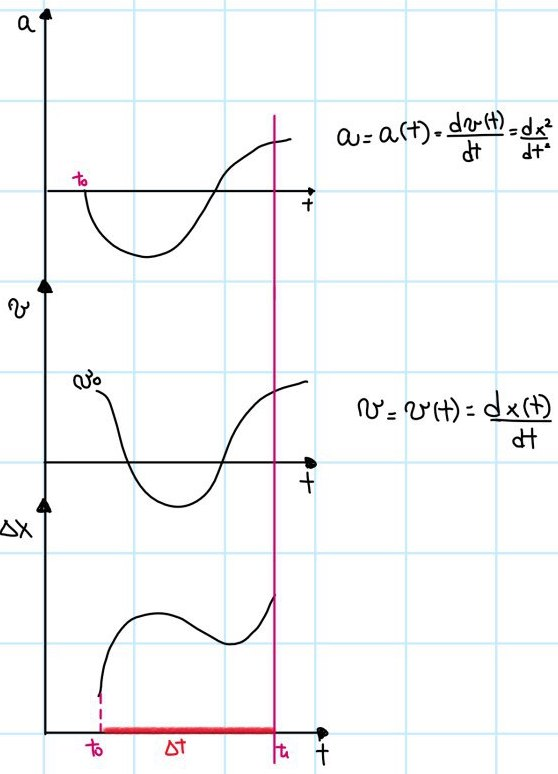
\includegraphics[width=0.50\textwidth]{1}
\end{center}
In questo grafico si osserva che quando si parla di accelerazione si fa riferimento
a quella istantanea \\
{\color{black} \rule{\linewidth}{0.3mm} }
\\ \\ 
Se per ipotesi avessimo l'accelerazione costante invece avremmo non più 
$\frac{\Delta x}{\Delta t}$ MA $\frac{\Delta v}{\Delta t}$, che rappresenta 
l'accelerazione media mantenendo per ovvio che
\begin{itemize}
	\item $\Delta t = t_{1} - t_{0}$
	\item $\Delta v = \Delta t \cdot a_{Media}$ 
	\item $\Delta v = v_{1} - v_{0}$
\end{itemize}
Si riesce a ricavare lo spostamento che a questo punto diventa 
\[\Delta x = v_{0}\Delta t +(\Delta v) \cdot \frac{\Delta t}{2} =
\Delta t \cdot \frac{v_{1}+v_{0}}{2} = \Delta t(v_{media})\]
A questo punto proviamo a ricavare la posizione $x_{1}$:
\[x_{1} = x_{0} + \frac{v_{1}}{v_{0}}{2}\cdot \Delta t\]
Dove in pratica $v_{1} = v_{0} + a_{Media} \cdot \Delta t$, sostituendo vien fuori
\[x_{1} = x_{0} \frac{v_{0}+a_{Media}\cdot\Delta t + v_{0}}{2} \cdot \Delta t\]
Se generalizziamo:
\[x(t) = x_{0} + v_{0}(t-t_{0})+\frac{a_{Media}}{2}(t-t_{0})^{2}\]
Successivamente, per finire, noteremo che:
\[x(t) = x_{0}+\int_{0}^{t}v_{0} dt + \int_{0}^{t} a_{media}t\cdot dt =\]
\[= x_{0} + v_{0}t + \frac{1}{2}at^{2}\]
\\ \\ \\ \\ \\ \\ \\ \\ \\ \\ \\ \\ \\ \\ \\ \\
{\color{black} \rule{\linewidth}{0.3mm} }
\paragraph{Illustrazione a cura di Letizia}
\begin{center}
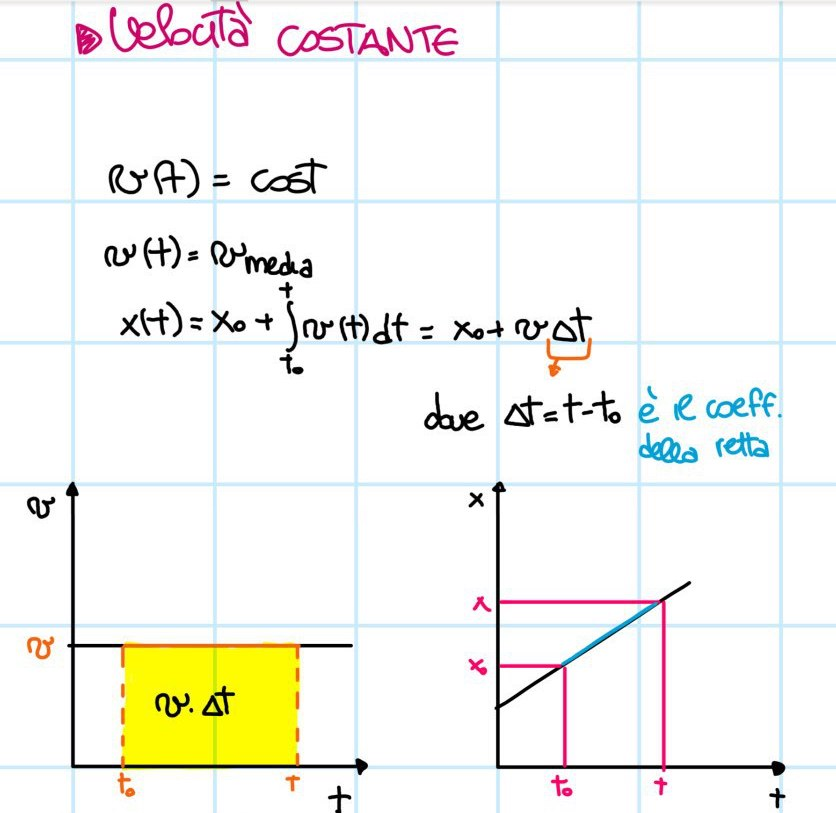
\includegraphics[width=0.75\textwidth]{vcostante}
\end{center}
In questo grafico si può osservare graficamente cosa accade quando si considera 
la velocità media come costante\\
{\color{black} \rule{\linewidth}{0.3mm} }
\chapter{Moto rettilineo uniformemente accelerato}
Dato qualsiasi piano inclinato, se un corpo parte dall'alto da un punto $x_{0}$
se esso rotola (con attrito volvente che è trascurabile), noteremo che con il
quadrato del tempo ($t^{2}$) la sua velocità si incrementerà
$x = x_{0} + v_{0}t + \frac{1}{2}at^{2}$, in cui possiamo giocare di nuovo a 
modificare le cose belle, tipo la t vi $v_{0}\cdot t$ può diventare 
$\frac{v-v_{0}}{a}$, da cui consegue che $a = \frac{v-v_{0}}{t}$ e quindi 
$x = x_{0} + \frac{1}{2}(v_{0}+v)\cdot t$.\newline
{\color{black} \rule{\linewidth}{0.3mm}}
\paragraph{Grafico dell'accelerazione costante}
\begin{center}
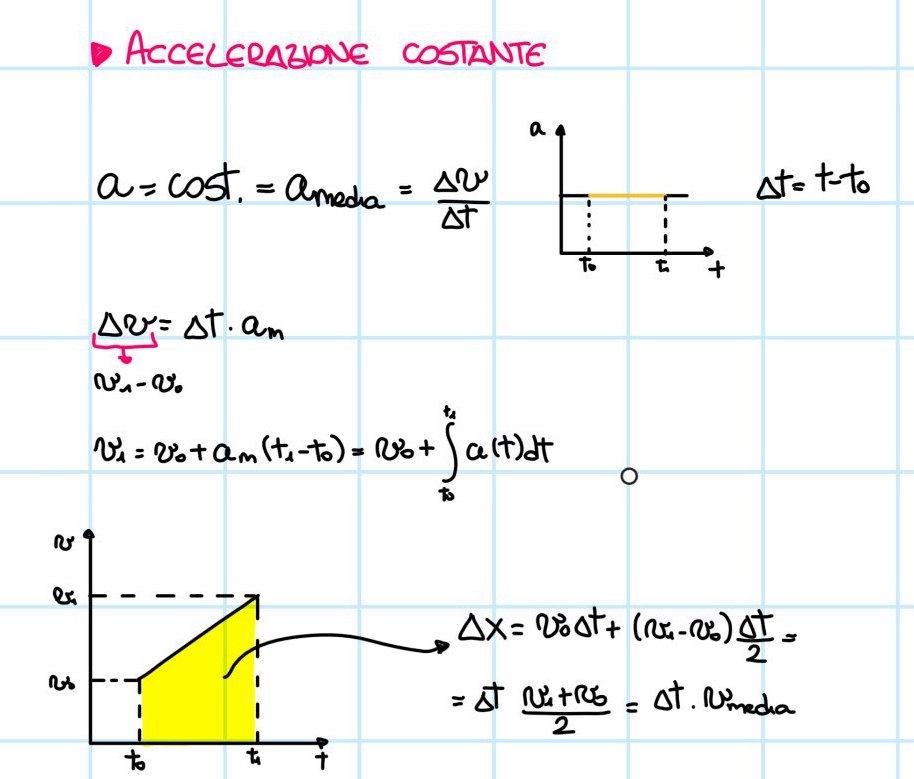
\includegraphics[width=0.75\textwidth]{acostante}
\end{center}
In questo grafico si nota che la variazione della velocità è coincidente con
la variazione del tempo per l'accelerazione media \\
{\color{black} \rule{\linewidth}{0.3mm}}
\section{Accelerazione di gravità}
Escludendo le forze di attrito con l'aria quando un corpo cade in caduta libera
si ottiene che esso (sul nostro pianeta) cada accelerando di 9,8 $\frac{m}{s^{2}}$.
Questi corpi prendono il nome di Gravi, e non importa che massa abbiano SE 
consideriamo l'assenza di aria che faccia attrito.
\\ \\
Poniamo caso di lanciare un sasso verso l'alto, o anche un mattone, MacBook, il
proprio gatto, quel che volete, noterete che questo salirà, e poi dopo un breve
periodo inizierà a tornare giù, questo è per via del fatto che l'accelerazione
gravitazionale è costante, ma all'oggetto che lanciamo cosa accade?
\\ \\
Noi sappiamo che $v = v_{0} + a\cdot t$, il grafico sarà una parabola che va
verso l'alto e poi ad un certo punto smetterà di crescere e inizierà a 
decrescere, e nel momento in cui il corpo scende l'accelerazione noteremo che
sarà $\leq$ 0 (Vettorialmente).
\paragraph{ATTENZIONE} L'accelerazione non si annulla MA sul punto di massimo
locale dove cambia il verso dell'accelerazione si avrà una velocità = 0
\chapter{Sistema cartesiano}
Il grafico di un qualsiasi sistema cartesiano è composto da due assi, uno x ed
uno y, perpendicolari tra essi, ed ogni punto sul grafico è composto da due
coordinate (x, y) tali che $P = (x_{P}, y_{P})$
\section{Coordinate polari} 
Ogni punto ha una distanza dall'origine, quella distanze si chiama R, e l'angolo
che si forma tra l'asse x e R si chiama $\phi$, di conseguenza ricaviamo che:
\begin{itemize}
	\item $\frac{y}{R} = \sin(\phi)$
	\item $\frac{x}{R} = \cos(\phi)$
	\item $y = R \cos(\phi)$
	\item $x = R \cos(\phi)$
	\item $\frac{y}{x} = \tan(\phi)$
	\item $\phi = \arctan(\frac{y}{x})$
	\item $R = \sqrt{x^{2}+y^{2}}$
\end{itemize}
Tutto ciò rimanendo comunque nel secondo quadrante, nel primo chiaramente c'è
da dire che rimane tutto cambiato di segno e viene indicato con le stesse lettere
del primo ma aggiungendoci un \' dopo.
\section{Somma tra vettori}
Dati due vettori è possibile individuarne la somma tramote la regola del 
parallelogramma che consiste nel tracciare due semirette parallele ai due 
vettori che abbiamo, e vanno aggiunte al termine del segmento del vettore
già presente, l'incrocio tra queste due semirette sarà il punto da cui puoi
calcolarti la somma (Non si capisce, ok, senza grafici è impossibile ma 
come già detto, li aggiungerò.) \\ \\ \\ \\
\\
{\color{black} \rule{\linewidth}{0.3mm} }
\paragraph{Letizia ci salva un'altra volta con un grafico}
\begin{center}
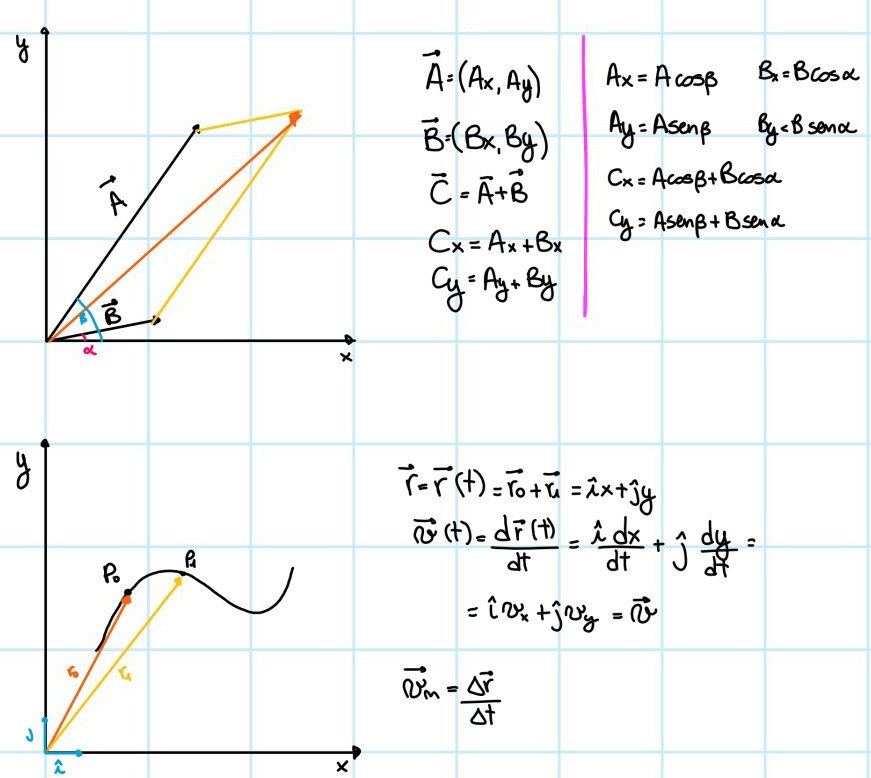
\includegraphics[width=0.75\textwidth]{sommaVettoriale}
\end{center}
%DESCRIZIONE DELL'IMMAGINE
Graficamente si verifica quello che ho scritto qui sopra. Si noti che tra l'altro
la velocità media
$\overrightarrow{v_{m}} è parallela (||) a \Delta \overrightarrow{r}$\\
e $\overrightarrow{v}=\frac{ds}{dt} \widehat{u}t $ (con u che sarebbe un 
versiore, ed s lo spazio), mentre per quanto concerne l'accelerazione 
$\overrightarrow{v}=\frac{dv}{dt} \widehat{u}t $ (Non c'è più s ma v che sarà
la velocità)
{\color{black} \rule{\linewidth}{0.3mm} }
\\
Se ragioniamo nelle due dimensioni la questione del nostro moto si complica, 
perchè abbiamo:
\[\overrightarrow{r} = \widehat{i}\cdot x + \widehat{j} y\] e quindi
\[\frac{d \overrightarrow{v} (t)}{dt} = \widehat{i} \cdot \frac{dx}{dt}+ 
\widehat{j} \cdot \frac{dy}{dt}\]
Scritto più easy: $\widehat{i} v_{x} + \widehat{y} = \overrightarrow{v}$

\[\overrightarrow{v_{Media}}= \frac{\Delta \overrightarrow{x}}{\Delta t} = 
\frac{\overrightarrow{r}}{\Delta t} \] dove $\Delta r = r_{1} - r_{0}$ e sarebbe
la distanza vettoriale.  \\ 
$\overrightarrow{v}(t) = \frac{\Delta \overrightarrow{r}}{\Delta t}$ con 
$\Delta t \to 0$
\\ \\ 
L'obbiettivo è quello di passare dal livello 1D al 2D, e la trigonometria entra
in gioco per via del fatto che vengono a formarsi dei triangoli
\\ \\
\\
{\color{black} \rule{\linewidth}{0.3mm} }
\paragraph{Illustrazione a cura di Simona}
\begin{center}
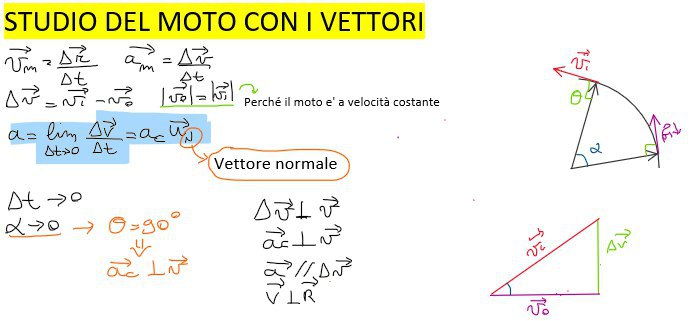
\includegraphics[width=0.75\textwidth]{mruvettoriale}
\end{center}
Da questo grafico è possibile notare in che modo interagiscono graficamente 
(considerando il punto di vista vettoriale) le velocità. 
\\
{\color{black} \rule{\linewidth}{0.3mm} }
\\
\section{Moto Circolare}
Consideriamo una circonferenza di raggio r, ed un punto materiale che si muove
lungo la suddetta circonferenza, che con l'asse x forma un angolo $\theta$. \\
\\
Supponiamo che il moto della velocità istantanea lungo la circonferenza sia 
costante, o meglio, diciamolo in modo figo: $\frac{dv}{dt} ~ costante$, se calcolo
l'accelerazione vettoriale, anche se il modulo è costante ma la direzione cambia
allora l'accelerazione non potrò mai esser nulla. 
\[\overrightarrow{a} = \frac{\overrightarrow{v}}{dt} \neq 0\]
\subsection{I vantaggi delle coordinate polari}
Introduciamo il concetto di radiante, ovvero date l, $\theta$ ed r,
\begin{itemize}
	\item Con r Raggio
	\item $\theta$ che è l'amgolo
	\item l che è la distanza NON vettoriale, cioè l'arco insomma tra due punti
\end{itemize}
Con $\theta = \frac{l}{r} = \frac{2 \pi r}{r} = 2 \pi$, pertanto si ottiene che
la velocità angolare $\omega$ sia = a $\omega = \frac{d \theta}{dt}$, e ricordiamo
che prima si era detto di essere in velocità costante, pertanto se moltiplichiamo
la velocità angolare per il raggio cosa otteniamo? Esatto, la velocità a cui
ci stiamo spostando, ovvero:
\[\omega R = \frac{dl}{dt} = v\]
Inoltre definiamo il concetto di PERIODO (t) che è il tempo impiegato per fare
tutto un giro della circonferenza: $T = \frac{2 \pi}{\omega}$, analizziamo
ora le leggi orarie
\[s(t) = s_{0} + v\cdot t\] Oppure
\[\theta(t) = \theta _{0} + \omega t\] a questo punto ragioniamo su quella
che è l'accelerazione vettoriale:\\ 
Sappiamo che $\overrightarrow{v_{m}} = \frac{\Delta \overrightarrow{r}}{\Delta t}$,
quindi ne deriva che $\overrightarrow{a_{m}} =
\frac{\Delta \overrightarrow{v}}{\Delta t}$ oppure in modo anche più preciso
\[\overrightarrow{a} = \lim \limits_{\Delta t \to 0} 
\frac{\Delta \overrightarrow{v}}{\Delta t} = a_{c} \widehat{u}_{n}\] in cui la
n specifica che è perpendicolare e non tangente, altrimenti sarebbe $\widehat{u}_{t}$, 
quindi si può concludere che l'accelerazione centripeta \[\overrightarrow{a_{c}}
= \frac{v^{2}}{r} \cdot \widehat{u}_{n}\] in cui ricordiamo che n indica che il 
versore sia PERPENDICOLARE, infatti la n sta per versore NORMALE.
Tutto questo se la velocità è costante.
\section{Moto circolare non uniforme}
Oltre all'accelerazione centripeta servirà l'accelerazione tangente o tangenziale
che è l'accelerazione lungo l'arco PERO' tangente alla circonferenza.
\[\overrightarrow{a_{t}} = \frac{d^{2}l}{dt^{2}}\cdot \widehat{u}_{t}\] E
si ricava che quindi $\overrightarrow{a} = \overrightarrow{a_{t}} \vee 
\overrightarrow{a_{c}}$, nel senso che è la stessa accelerazione ma considerata
da due sistemi di riferimento diversi. \\
Di conseguenza se è uniformemente accelerato, possiamo
anche stabilirne la legge oraria, che è simile a prima: 
\[l(t) = l_{0} + v_{0}t + \frac{1}{2} \cdot a_{t}t^{2}\], che è di base, mentre
nel caso andiamo a considerare le velocità angolari.
\[\theta(t) = \theta _{0} + \omega _{0}t + \frac{1}{2} a_{\omega}t^{2}\]
Se prima si è considerata la velocità normale ora consideremo quella tangenziale, 
ma alla fine, in un caso vedavamo quanto ci si era spostati, nel secondo caso
si vede quanto si è allargata o ristretta la circonferenza. Perchè? 
Perchè \textbf{la circonferenza è l'insieme di tutti i punti equidistanti da un punto
detto centro}.
\section{Circonferenza e Moto Armonico}
Prendendo una qualsiasi circonferenza ed un punto P su di essa, è possibile 
tracciare sull'asse x ed y i punti relativi a P, e ne consegue che
\[x = R\cos \theta = R\cos(\omega t) e \\
y = R\sin \theta = R\sin(\omega t) \] 
E quindi 
\[\frac{dx}{dt} = \omega R \cdot \sin(\omega t) \] e
\[\frac{dy}{dt} = \omega R \cdot \cos(\omega t) \]
Inoltre \[v = \sqrt{\frac{dx^{2}}{dt} + \frac{dy^{2}}{dt}} \]
\\
{\color{black} \rule{\linewidth}{0.3mm} }
\\
\paragraph{Illustrazione a cura di Simona}
\begin{center}
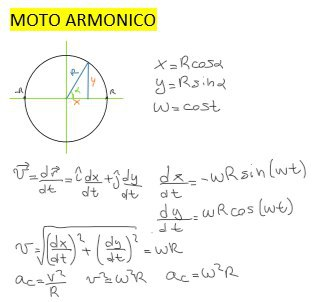
\includegraphics[width=0.75\textwidth]{motoarmonico}
\end{center}
In quest'illustrazione si vede riassunto graficamente quello che ho menzionato
nel paragrafo superiore \\
{\color{black} \rule{\linewidth}{0.3mm} }
\\
Finalmente si può rispondere alla domanda che ci si è fatti all'inizio: ovvero,
come posso calcolare la traiettoria di un corpo BASANDOMI sulle forze che 
agiscono su di esso?\\ \\ 
Introduciamo pertanto il concetto di trasformazione Galileiana
\section{Trasformazione Galileiana} 
Il primo passo è sempre avere un sistema di riferimento a coordinate, ma di 
questi ne esistono infiniti, pertanto sarà importante rimanere nello stesso 
sistema di riferimento, nel senso che tutto varia in base a quello. \\ \\
Ad esempio, supponiamo di avere 3 posizioni di 3 corpi diversi. 
\begin{itemize}
	\item A: Un'automobile
	\item P: Un pedone
	\item B: Una bicicletta
\end{itemize}
E di conseguenza le distanze tra essi $\overrightarrow{X_{BA}}, 
\overrightarrow{X_{PA}}, \overrightarrow{X_{PB}}$, noi possiamo dedurre che:
$v_{PB} = \frac{dx_{PB}}{dt} = v_{AP} + v_{AB}$. \\ \\
Se queste sono velocità da considerarsi vettoriali ($\overrightarrow{v_{PA}}$), 
siccome i punti sono in serie sullo stesso piano, allora basta fare semplicemente
la somma. 
\paragraph{Detto in modo più umano: } Siete in macchina, andate a 70$\frac{km}{h}$,
vi supera una macchina che va a 130$\frac{km}{h}$, ecco, dal punto di vista
della velocità abbiamo appena detto che è come essere fermi, e una macchina va
a 60$\frac{km}{h}$, dipende dal vostro sistema di riferimento.
\\ \\
\chapter{La Forza}
Finora abbiam descritto le accelerazioni per esempio di un corpo in caduta 
libera, abbiam descritto COME un oggetto cade, ma nessuno ha risposto al perchè
l'oggetto cade. Prima ci si chiedeva perchè c'è movimento? \\ \\
Perchè alcuni oggetti si muovono senza una causa? Esempio lampante: La Luna,
si muove (da un pochino di tempo anche) da sola, senza nessuno che spinge.
\paragraph{Consiglio: } Guardatevi questo spettacolo a teatro di Paolini che 
parla di Galileo, io l'ho adorato, anche se mi rendo conto che in sessione non
avrete per nulla voglia di guardare qualcosa di questo genere ->
\href{https://www.youtube.com/watch?v=8alJ9eFl634}{This}
\\
{\color{black} \rule{\linewidth}{0.3mm} }
\\
Ora, da una parte abbiamo le forza che sono descrivibili con delle formule, 
e dall'altro abbiamo la meccanica che vuole sapere cosa fanno le nostre forze
al punto materiale che le subisce. Ammesso che capisco quanto valga una forza, 
cos'è una forza?
\paragraph{Definizione: }Da \href{https://it.wikipedia.org/wiki/Forza}{Wikipedia}: 
Una forza è una grandezza fisica 
vettoriale che si manifesta nell'interazione reciproca di due o più corpi, sia 
a livello macroscopico, sia a livello delle particelle elementari. Quantifica il 
fenomeno di induzione di una variazione dello stato di quiete o di moto dei corpi 
stessi; in presenza di più forze, è la risultante della loro composizione vettoriale
a determinare la variazione del moto. La forza è descritta classicamente dalla 
seconda legge di Newton come derivata temporale della quantità di moto di un
corpo rispetto al tempo \\ \\
All'atto pratico una forza è quella che causa il movivmento, di fatto se si 
applica una forza, o comunque ci sono delle forze che agiscono su di esso, allora
quest'ultimo si muoverà, o per esser più preciso Accelera. Essendo una grandezza
vettoriale, se la somma algebrica delle forza applicate su un corpo è = 0 allora
il corpo avrà accelerazione 0. \\ \\ \\
\footnote{Lamentela personale}Credo di volermi rifiutare di fare menzione della 
definizione dataci a lezione con l'esempio della molla. Ditemi voi se è ammissibile 
una definzione del tipo "Una forza è quella esercitata da una molla quando la tiri 
o comprimi". 
\\ \\
Detto in modo più matematico, primo principio della dinamica (\textbf{principio di inerzia}):
\[
Se~~\overrightarrow{F} = \sum_{\kappa=1}^n \overrightarrow{F_{\kappa}} = 0
~~ allora ~~ a = 0
\]
Se su un corpo non agisce alcuna forza viene mantenuta costante la propria 
velocità, pertanto essa può essere anche $\geq 0$, ma rimarrebbe costante per
via dell'assenza di forze che si oppongono al movimento.
\\ \\
Esatto, perchè potrebbe accadere che esistano forza che non agiscono direttamente
come quella centripeta, quella di gravità, quella centrifuga, è pieno di forze
che agiscono indirettamente. Sono forze che compaiono nel sistema di riferimento
non inerziale.
\\ \\
\section{Secondo principio della dinamica}
Dato un corpo fermo, in base al suo peso dovremo applicare una forza maggiore o
minore, per ottenere una determinata velocità. Cioè se devo spingere una penna, 
e farla viaggiare a una velocità $\lambda$, è ben diverso far raggiungere la
stessa velocità $\lambda$ ad un camion. (Ponendo $\lambda > 0$) \\ \\
Da questo consegue che la massa influenza sia l'accelerazione che la forza.
Infatti il secondo principio della dinamica dice che:
\[
F = m\cdot A
\]
Provocare dell'accelerazione in un corpo richiederà più o meno forza in base
alla massa del corpo da spingere. Ne consegue che:
\[
m_{x} = m_{0} \cdot \frac{a_{0}}{a_{x}}
\]	
Chiaramente c'è da dire che un qualsiasi corpo, se è fermo necessiterà di 
applicare più forza per produrre un determinato movimento, se spingiamo un corpo
che già si muove ci vorrà meno forza.
\paragraph{La Massa: } Anche se la si dà per scontata, non l'abbiamo definita in
modo specifico, è considerabile al momento come quantità di materia, pertanto
mi raccomando da ora non confondiamo più massa e peso.
\paragraph{Il Peso: } Il peso è una forza, che è esercitata dal campo gravitazionale
terrestre ed è di circa 9,8 N (dove N sarebbe Newton). Il peso è una forza, è una
grandezza vettoriale, ha una direzione, un verso, ed un modulo o intensità.
\paragraph{Precisazione: } Nella meccanica classica tendenzialmente una forza è
realizzabile/applicabile/esistente SE son presenti due corpi, pertanto ci si può
anche esprimere dicendo che: Presenza di forze $\to$ presenza di più corpi. \\ \\
In assenza di forza non si ha accelerazione, pertanto lo stato di moto di un
punto materiale è o a 0 o velocità costante, di fatto nel mondo in cui viviamo,
in quello reale ci sono sempre delle forze che agiscono, e appare che i corpi
non abbiano velocità costante. \\ \\
Questo è dovuto per esempio alle forze di attrito che ci sono sempre, cose
di questo tipo. \\ 
Per tastare con mano quello che è un moto perfettamente (o quasi) costante, si 
può osservare il movimento della luna, che ok, non è perfettamente nel vuoto 
anche perchè il vuoto assoluto non esiste, però non ha degli attriti così consistenti.
\\ \\
Il principio (detto principio di inerzia) si basa sul concetto del "In assenza
di forte il corpo conserva il suo moto", o meglio, se non ci sono corpi vicini
che influenzino un corpo allora la sua accelerazione sarà = 0 .
\section{Quantificare una forza}
L'unità di misura di una forza è il Newton (N), \\
Se il corpo pesa 1kg si ha che: 1 N = $1m/s^{2}\cdot kg$ pertanto $F(t) \alpha a(t)$,
cioè la forza applicata in un tempo è proporzionale all'accelerazione in quel
determinato tempo. 
\begin{itemize}
	\item [m] = kg
	\item [a] = $\frac{m}{s^{2}}$
	\item [F] = kg $\frac{m}{s^{2}}$ = N 
\end{itemize}
Ovviamente (come specificato prima) anche $\sum_{i=1}^n
\overrightarrow{F_{i}} = 0 \to \overrightarrow{a} = 0$, e quindi ad esempio:
\[
\begin{cases}
m_{0} = 1kg \to a_{0}\\
m_{1} = \lambda kg \to a_{1}
\end{cases}
\]
$\frac{m_{0}}{m_{1}} = \frac{a_{0}}{a_{1}}$, e quindi questo significa che 
ragionando per formule inverse $m_{1} = m_{0}\cdot \frac{a_{1}}{a_{0}} \forall F$
\\ \\
Non si è specificato, MA la somma di due masse è fattibile, cioè se prendo 
una mela e una pera e le incollo, la loro massa sarà $mela + pera + colla$, 
pertanto l'accelerazione seguira questa somma, nel senso, se ho calcolato
l'accelerazione prima che avrebbe la mela, poi la pera, la loro somma avrà un 
valore approssimativativamente proporzionale alla somma delle masse (circa perchè
c'è la colla ma è diciamo trascurabile.)
\\ \\
\paragraph{Riprendendo il secondo principio della dinamica: }
Ricordiamoci la difficilissima formula $F = m \cdot a $, e quindi 
$\overrightarrow{F} = m \cdot \overrightarrow{a}$. \\ \\
Il problema è che io data una forza posso concludere di avere una massa per un'accelerazione MA
non posso concludere data una massa ed accelerazione che ci sia quella forza.
Non mi sta definendo la forza, è una sua espressione. Ti serve una teoria sulla
forza per lavorarci su. In termini più semplici: Da sinistra verso destra l'equazione 
$\overrightarrow{F} = m \cdot \overrightarrow{a}$ va bene MA da destra verso
sinistra no. Un esempio di alternativa a questo? 
\paragraph{Legge di Gravitazione Universale}
\[\overrightarrow{F_{a}} = G \cdot \frac{M\cdot m}{d^{2}}\] in cui la G è la
costante di gravitazione universale ed è $g = \frac{G\cdot M}{R_{Terra}^{2}}$, 
g invece è la forza g, quella che si vede di solito in F1 in curva o frenata, in
cui letteralmente si hanno decelerazioni e accelerazioni (non necessariamente 
rettilinee, generalmente più in curva) fino ai 5g. \\ \\
Inoltre, siccome questa g dipende dal raggio della $terra^{2}$, quindi può 
cambiare anche sulla terra stessa.
\section{La Molla}
La molla è un tipo di corpo su cui si può applicare sia una compressione che 
un'espansione, ma attenzione, non si chiamerà più espansione ma allungamento, 
perciò essendo un corpo, su di esso si può applicare una forza. \\ \\
Sulla molla si può applicare una forza sia tirandola che spingendola, e questa
forza è:
\[
\overrightarrow{F_{k}} = -k \cdot (\overrightarrow{x} - \overrightarrow{x_{0}})
\]
In cui $\overrightarrow{x} - \overrightarrow{x_{0}}$ sui libri di fisica vien
chiamata $\Delta l$ e sarebbe l'allungamento, o quanto s'è deformata la molla.
\\ \\
\section{Il peso}
Siccome misurare il rapporto tra masse è uguale a misurare il rapporto tra forze,
allora si conclude che si ha la stessa gravità, che sulla terra è 9,8, e quindi
si può anche dire che per misurare una massa, bisogna tener conto della forza peso 
e confrontarla con la gravità che si sta considerando.
\[\overrightarrow{P} = m \overrightarrow{a} = m \overrightarrow{g} = - m\cdot 
g \cdot \widehat \gamma\]. 
Se una bilancia misura una forza, dato g, si ottiene che $\frac{forza}{g} = massa$,
per cui se è vero che il peso cambia in base a dove ci troviamo, non è vero
che lo faccia anche la massa, e infatti la massa quella è e quella rimane.
\section{Terza legge della dinamica}
E' anche detto principio di azione/reazione, ovvero:
\paragraph{Definizione: } Dati due corpi, per qualsiasi forza che viene applicata 
da un corpo all'altro (per ogni azione), corrisponderà una forza (reazione) che
sia uguale e contraria $\to azione(corpo_{a}, corpo_{b}) = 
reazione(corpo_{a}, corpo_{b}) = azione(corpo_{b}, corpo_{a})$ \\ \\
Questo principio è diretto derivante dall'interazione tra due oggetti, due corpi,
e con questa consapevolezza si deduce che (oltre al discorso della presenza di
più corpi) si avranno anche delle ulteriori forze dovute ad attriti etc. \\ \\
L'azione e reazione sono chiaramente esercitate dipendentemente da chi applica
forza su chi. Nel senso, se io pesto un pugno sul tavolo, io agisco, il tavolo
reagisce, io perisco la reazione del tavolo e sento dolore.\\ \\
La somma di tutte le forze che agiscono su un corpo è $$\overrightarrow{F_{A}}
= \sum_{i=1}^{n} \overrightarrow{F_{A_{i}}} = m \cdot \frac{d^{2}
\overrightarrow{x_{A}} (t)}{dt^{2}} = m\cdot \overrightarrow{a_{A}}$$ In cui, 
per non confonderci specifico che in questa formula 
\begin{itemize}
	\item A = nome del corpo
	\item a = accelerazione
	\item $d^{2}$ = derivata alla seconda
	\item $t^{2}$ = letteralmente t al quadrato
\end{itemize}
\paragraph{Forza normale}
Supponiamo di avere un tavolo T ed un corpo di massa M, un cubo, per intenderci.
E ricordiamo che il tavolo sta al di sopra della terra, che chiameremo TE. 
(Mantenendo per ovvio che in questo caso la gravità si possa considerare 
costante $\to F_{G} = G \cdot \frac{M_{Terra \cdot M}}{R_{Terra}^{2}}$)
\\
{\color{black} \rule{\linewidth}{0.3mm} }
\begin{center}
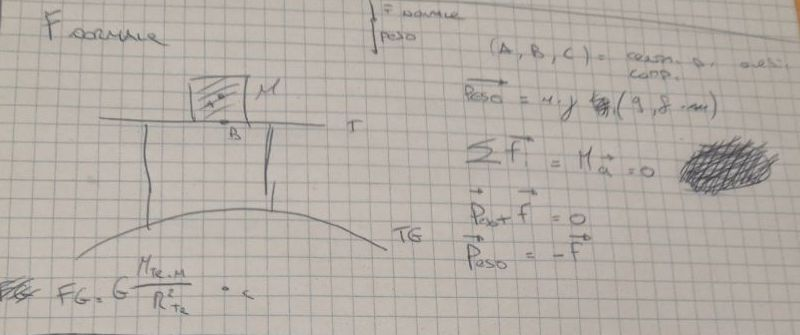
\includegraphics[width=0.75\textwidth]{forzanormale}
\end{center}
In breve, sulla massa agiscono ben due vettori, e pure sul tavolo agiscono più
vettori, in quanti agiscono sia l'azione della forza peso che la reazione del 
cubo. \\ \\
In italiano: Sul tavolo c'è il peso del cubo, il tavolo esercita peso sulla terra,
ed esercita azione su cubo. \\ \\
La domanda è: Perchè questi corpi rimangono fermi? La somma di tutte le forze
è uguale a zero, quindi l'accelerazione è 0, quindi stanno fermi.
\paragraph{Precisazione:} La massa non esercità forza peso, ma è la forza peso
che viene esercitata sulla massa.
\\
{\color{black} \rule{\linewidth}{0.3mm} }
\\
Il concetto di azione e reazione funziona perfettamente, ma bisogna sempre
ricordarsi del fatto che le forze vengano applicate da due corpi distinti.
\section{Il lavoro di una forza}
Il lavoro è il legame tra lo spostamento di un corpo per la quantità di energia
spesa per muoverlo. Attenzione, non è in generale quanto è lo sforzo, MA è quanto
movimento viene prodotto grazie ad una determinata forza. \\ \\
Più semplicemente, se tendo di spostare un pallone da calcio, applico una forza,
si muove, ergo compio del \textbf{lavoro}. \\ \\
Se tento di spostare l'Empire State Building, oltre a far la figura del deficiente,
ottengo che quest'ultimo malgrado applico l'incredibile forza dei miei muscoli,
non si muove, sta fermo, quindi il lavoro sarà 0.
\\  \\
Più precisamente:
\[L = F \cdot \Delta x\]
Forza x spostamento, molto semplicemente, ma occhio a non confondersi, poichè
spostamento e forza sono grandezze vettoriali ($\overrightarrow{F}, 
\overrightarrow{\Delta x}$)
\\ \\
L'unità di misura del lavoro è il Joule (J), che coincide con $N\cdot M$, e come
è possibile notare questo è uno \textbf{scalare} nel senso che (Raga, in algebra
io 'sta roba non l'avevo ancora capita.) il prodotto di due vettori è uno scalare.
\\
{\color{black} \rule{\linewidth}{0.3mm} }
\begin{center}
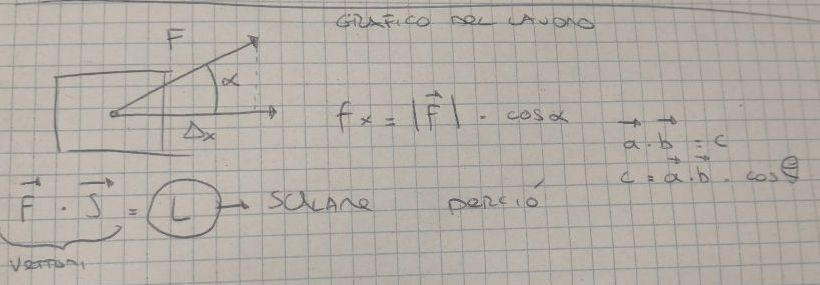
\includegraphics[width=0.75\textwidth]{graficoLavoro}
\end{center}
{\color{black} \rule{\linewidth}{0.3mm} }
\\
Avendo definito il lavoro, con questa definizione abbiamo una quantità che 
consente di definire il quantitativo di energia trasferito in un sistema
dall'esterno verso l'interno di un sistema. \\ \\
E se invece fossero più forze a generare uno spostamento? Cioè molto semplicemente,
se spostiamo un tavolo in due invece che da solo? Beh cambia molto lo 
spostamento, e infatti \[L = \sum_{i=1}^{n} \overrightarrow{F_{i}} \cdot \overrightarrow{S}\]
Ah ovviamente $L_{i} = \sum_{i=1}^{n} \overrightarrow{F_{i}} \cdot \overrightarrow{S}$,
da questa prospettiva si conclude anche che $L_{tot} = \sum_{i=1}^{n} L_{i}$.
\\ \\
Infine, altro modo di esprimere il lavoro:
\[L_{\kappa} = \int_{a}^{b} F_{\kappa}dx  \]
Quindi chiaramente è possibile dire che:
\[L = \int_{a}^{b} F(x) dx\]
Ossia, nel caso prima semplicemente abbiamo specificato un punto preciso MA,
se ragionassimo con $\overrightarrow{F}$ per ottenere il lavoro totale manca un
piccolo passaggio:
\[L = \int F(x) dx + \int F(y) dy + \int F(z) dz = \int \overrightarrow{F}\cdot 
d \overrightarrow{s}\]
{\color{black} \rule{\linewidth}{0.3mm} }
\begin{center}
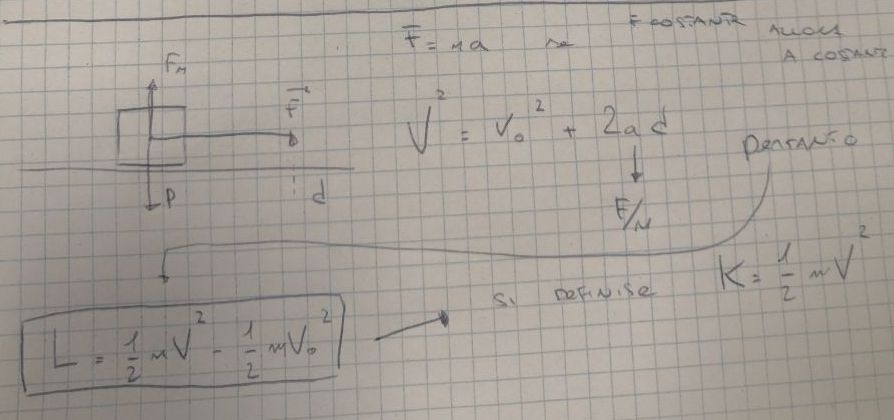
\includegraphics[width=0.75\textwidth]{velocitalavoro}
\end{center}
In questo caso cosa si osserva? La velocità al quadrato che avremo sarà coincidente
con la velocità iniziale alquadrato, che si somma con la velocità generata
dall'accelerazione provocata dalla applicazione della forza in questione.\\ \\
Quel K si chiama \textbf{ENERGIA CINETICA}, ossia l'energia associata al moto. Mi raccomando,
contate sempre che ci sono altre energie in questione che agiscono su un corpo
in movimento, allora tutto prende senso. (in seguito sarà approfondita nello
specifico)
\\
{\color{black} \rule{\linewidth}{0.3mm} }
\chapter{Principio di conservazione dell'energia}
E' il classico esempio del modo di pensare dei fisici, cioè osservi un fenomeno,
noti qualcosa di anomalo, lo testi, trai delle conclusioni, ma in questo caso
addirittura vengono inventate delle unità di misura.
\\ \\
Il concetto di Energia è risultante da calcoli che effettuiamo MA NON ESISTE, 
l'energia NON è fisica, non è qualcosa di tangibile, è CALCOLABILE, e rimane
nel tempo sempre uguale a se stessa in determinate situazioni. \\ \\
Se nel caso della meccanica e dinamica si aveva qualcosa di misurabile, tangibile,
per quanto riguarda la conservazione dell'energia si dovrà capire il concetto di
sistema.
\paragraph{Cos'è un sistema: } E' un insieme di punti materiali (può essere 
pure uno solo), può essere contenuto in un sistema, ovviamente.
\\ \\
Alla fine si ha una quantità di Energia, che viene associata al sistema, è
una serie di formule che vedremo, ma prima di applicarle devo capire bene quale
è il mio sistema di riferimento.\\ \\
Neanche a dirlo ci sono diversi tipi di energia, diciamo infinite forme da questo
punto di vista ad esempio:
\begin{itemize}
	\item Calore
	\item Cinetica
	\item Nucleare
	\item Chimica
\end{itemize}
Quello di cui ci occuperemo nello specifico per ora è l'energia cinetica.
\section{Energia Cinetica}
L'energia cinetica è (come detto sopra) l'energia che si associa al moto, o 
meglio l'energia che ha un corpo in movimento. Diciamoci subito le formule utili:
\begin{itemize}
	\item $L = \Delta \kappa$
	\item $\kappa = \frac{1}{2}m\cdot v^{2}$
	\item $L = \sum_{i=1}^{n} L_{i}$
	\item $L = \sum_{i=1}^{n} \overrightarrow{F_{i}} \cdot \Delta
	\overrightarrow{x} (Spostamento)$
\end{itemize}
Lavoro ed energia cinetica sono strettamente legati per via del fatto che 
appunto il lavoro è il prodotto di una forza per uno spostamento. Per cui \\
\[
L = \int_{x_{iniziale}}^{x_{finale}} F(x) dx = 
\int_{x_{iniziale}}^{x_{finale}} m\cdot a ~ dx
\]
A questo punto osserviamo che l'accelerazione è: $a = \frac{dv}{dt}$, quindi 
la formula è riscrivibile come \[L = \int_{x_{iniziale}}^{x_{finale}} m\cdot v 
\cdot \frac{dv}{dt} dx\] 
Ora le cose iniziano un po' a complicarsi, perchè se per ipotesi noi considerassimo
soltanto la velocità si avrebbe: $L = \int_{x_{iniziale}}^{x_{finale}} m\cdot v 
= \frac{1}{2}m\cdot v^{2}$\\ \\
Tutto sto casino è per arrivare a dire che: 
\[\frac{1}{2}m\cdot v_{finale}^{2} - \frac{1}{2}m\cdot v_{iniziale}^{2} = 
\Delta\kappa\]
Ecco, questo $\Delta\kappa$ è la variazione dell'energia che c'è stata da un 
punto iniziale ad un punto finale. \\ \\
Ora la domanda è: se ho compiuto un lavoro, perchè $\Delta\kappa$ è = 0? Perchè
non stiamo considerando tutte le altre forze! \\
\\Se io prendo il mio telefono e lo
striscio sul tavolo da un punto A ad un punto B, questo si ferma, MA per via
della forza di attrito. \\ 
\\
{\color{black} \rule{\linewidth}{0.3mm}}
\\
Da un punto di vista "Telemetrico" l'azione delle forze sul telefono che ho 
strisciato sul tavolo è di questo tipo:
\begin{center}
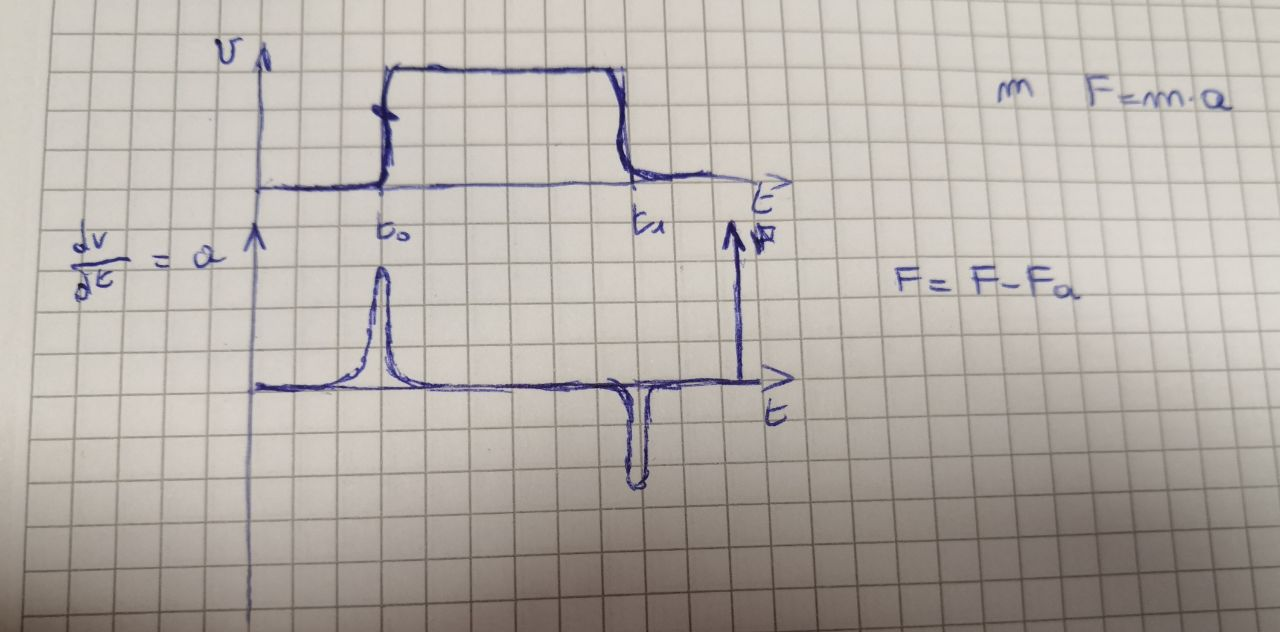
\includegraphics[width=0.75\textwidth]{telefonoStriscia}
\end{center}
Il primo grafico indica l'energia cinetica del telefono (che poraccio lo stiamo
massacrando a furia di sballottarlo in giro), mentre invece il grafico di sotto
indica come si comporta l'attrito che lo frenerà.\\ \\
(Per capire meglio cosa succede in un contesto del vuoto, ai videogiocatori 
consiglio di giocare \href{https://store.steampowered.com/app/244850/Space_Engineers/}
{Space Engineers}. E' bello, fidatevi.) \\ \\
\end{document}
